\documentclass[11pt]{article}

\usepackage{amsmath}
\usepackage{amssymb}
\usepackage{amsfonts}
\usepackage{amsthm}
\usepackage{backnaur}
\usepackage[scaled]{beramono}
\usepackage{bm}
\usepackage[small,bf]{caption}
\usepackage[strict]{changepage}
\usepackage{dblfloatfix}
\usepackage{enumerate}
\usepackage{enumitem}
\usepackage{flushend}
\usepackage[T1]{fontenc}
\usepackage{graphicx}
\usepackage{ifsym}
\usepackage{lipsum}
\usepackage{listings}
\usepackage{makeidx}
\usepackage{mathrsfs}
\usepackage{multirow}
\usepackage{pdfpages}
\usepackage{subcaption}
\usepackage{setspace}
\usepackage{textcomp}
\usepackage[hyphens]{url}
\usepackage{booktabs}
\usepackage{multirow}
\usepackage{xcolor}
\usepackage{pgfgantt}
\usepackage{wrapfig}
\usepackage{balance}
\usepackage{tikz}
\usetikzlibrary{shapes,decorations}
\usepackage{pgfplots}
\usepgfplotslibrary{units}
\pgfplotsset{compat=1.14}
\usepackage{bm}
\usepackage[
backend=biber,
style=ieee
]{biblatex}
\usepackage{hyperref}
\hypersetup{
    colorlinks=true,
    linkcolor=blue,
    filecolor=magenta,
    urlcolor=cyan,
}
\addbibresource{references.bib}

\newcommand{\rt}{\textsuperscript{\textregistered}}
\newcommand{\tm}{\texttrademark}

\addtolength{\evensidemargin}{-.5in}
\addtolength{\oddsidemargin}{-.5in}
\addtolength{\textwidth}{0.8in}
\addtolength{\textheight}{0.8in}
\addtolength{\topmargin}{-.4in}
%%%%%%%%%%%%%%%%%%%%%%%%%%%%%%
%%%%%%%%%%%%%%%%%%%%%%%%%%%%%%
%%%%%%%%%%%%%%%%%%%%%%%%%%%%%%
\title{\vspace{-25pt}
\huge CS 15-618 Project Report \\
\huge Synchrony (ID 24)
}
\author{
    Patricio Chilano (pchilano) \\
    Omar Serrano (oserrano)
}
\date{\today}

\begin{document}

\definecolor{beaublue}{rgb}{0.74, 0.83, 0.9}

\lstset{
    language=C++,
    basicstyle=\ttfamily\scriptsize,
    keywordstyle=\color{blue}\ttfamily,
    stringstyle=\color{red}\ttfamily,
    commentstyle=\color{orange}\ttfamily,
    morecomment=[l][\color{magenta}]{\#},
    breaklines=true,
    morekeywords={nullptr,noexcept},
    xleftmargin=.1\textwidth,
    xrightmargin=.1\textwidth,
}

\maketitle

\section{Summary}
We implemented a set of serial and concurrent linked lists and hash maps using
different synchronization mechanisms, including coarse-grained locks,
fine-grained locks, fine-grained spinning-reader-writer locks, and lock free. We
then compared the performance of these data structures under different
use-profiles. Finally, we compared the performance of our hash maps with Intel's
Thread Building Block's (TBB) and libcuckoo's concurrent hash maps under different
use-profiles.

\section{Background}

\subsection{Linked List} \label{ssec:bglist}
Linked lists are a simple data structure that is simply made up of zero or more
nodes connected in serial via pointer links, where each node contains a data
value, and a link to the next node. The basic operations they support are
insertion, removal, and lookup. Insertions take an input data value, create a
new node with the data value, and insert the node somewhere in the list,
typically the front or back of the list. Removals take an input data value,
search for a node containing the item, and remove the node from the list.
Lookups take an input data value, search for a node containing the value, and
return a reference/pointer to the data value or the node containing the value.

Linked lists are not inherently parallel, because typically operations begin at
the head of the list, and so there is an intrinsic bottleneck; however,
enhancing a linked list's concurrency is still worthwhile the effort because
they are convenient to use and are often the foundation for other data
structures which we might also need to be concurrent, such as stacks, queues,
hashmaps, skip-lists, etc. Furthermore, many algorithms rely on {\em list-like}
data structures, e.g., depth-first search uses a stack for the list of nodes in
the frontier, and to make them concurrent it may be necessary to start with the
list. Note the emphasis on {\em list-like}, because in some cases it may be
preferable to use an array.

The first concern in making a list concurrent is making it thread-safe. This is
easliy accomplished by locking the whole list for any operation, but prevents us
from exploiting parallelism. Despite the lack of a parallel-friendly nature,
there is still plenty of opportunity to parallelize operations on a linked list,
especially if different threads work on different nodes. Ideally, read-only
operations should be completely parallel, but even modify operations can be
parallel if nodes to be modified are not neighbors. Ultimately, to parallelize
operations on a linked list we must use some kind of synchronization technique
to avoid corrupting the list. It is with this in mind that we decided to implement
a set of concurrent lists and hashmaps using different synchronization techniques,
including a lock free list, and lists with coarse-grained, fine-grained, and
fine-grained spinning-reader-writer locks. Our goal was to learn to implement
these techniques, and to learn how these techniques fare under different kind of
workloads and use-profiles, i.e., the characteristics of how it is used, such as
percent of insertions, lookups, and removals.

In theory, each technique has it's own set of advantages and disadvantages.
Coarse-grained locks are easy to implement and only require one lock per list,
but each operation locks the whole list and prevents parallelism. Fine-grained
locks offer more opportunity for parallelism, but are more difficult to
implement than coarse-grain locks, require one lock per node, and increase the
cost of traversing the list, because every hop requires locking a node.
Fine-grained spinning-reader-writer locks have similar characteristics to
regular fine-grained locks, with the difference being that they support multiple
readers, bus contention becomes an issue, and fairness can become an issue for
writers if there are only a few of them but there are many readers. Lock free
lists, on the other hand, don't use locking. They rely on atomic
compare-and-swap (CAS) operations, and for this reason are more difficult to
implement, but offer the greatest degree of parallelism because no thread is
prevented from making progress.

\section{Technologies used}
\subsection{Language}
We used C++11 because it would allow us to work at a high level of abstraction,
making it easy for us to think about lists and nodes as objects, while also
allowing us to work close to the metal, allowing us to control memory allocation
and directly reference memory addresses. C++11 overloaded operators makes it
easy to work with atomic primitives, and this proved useful for implementing a
spinning-reader-writer lock, and the lock-free list. It is also much easir to
work with C++11's threads rather than pthreads, because C++11 allows you to
supply the thread with any callable object, including pointers to member
functions, and a variable number of arguments of any type.

\subsection{Target machines}
Our target machines were latedays cluster and GHC machines. Clearly, they are
convenient because we have access to them, but they are also a good choice
because they are relatively modern in terms of architecture and CPU model, they
are Linux machines, which is a system-level programming friendly OS, and they
have a decent number of cores, enough to see clear patterns in our experiment
results. Furthermore, the latedays cluster is ideal to run experiments because
it allowed us to run multiple jobs on different machines simultaneously. Our
initial plan was to use a single machine in the latedays cluster, but it became
evident that we would need to split the jobs among the machines, otherwise the
jobs would timeout, even with 8 hours of walltime. We conducted experiments on
both the GHC and latedays cluster machines, but most of the results presented
here are from the latedays cluster.

\subsection{External libraries}
In addition to comparing the different synchronization techniques we also wanted
to compare our concurrent data structures with an external library to get an
idea of the caliber of our implementation, and ofcourse for fun as well! We were
not able to find in time a library that implemented a plain vanilla concurrent
linked list (TBB implements concurrent deques and vectors, but not a list), but
we did compare TBB's and libcukoo's concurrent hash map with ours.

% Also used GoogleTest lib

\section{Approach}

\subsection{Overview}
At a high level, our approach consisted of the following steps:
\begin{enumerate}
\item
Implement a serial linked list.
\item
Implement a template hashmap where the bucket type is parameterized.
\item
Implement concurrent linked lists with the synchronization mechanisms listed in
section~\ref{ssec:bglist}.
\item
Create hashmaps with different bucket types by plugging in the lists to the
template hashmap.
\item
Create serial and asynchronous correctness tests for the lists and hashmaps.
\item
Create a benchmarking harness to test the lists and hashmaps, including TBB and
libcuckoo hashmaps, with different use-profiles.
\end{enumerate}

\subsection{Serial linked list}
The most important aspect of our serial linked list is the interface we chose to
implement, depicted in figure~\ref{fig:dllist}. Our goal was to make it simple
to test insertions, lookups, and removals, and we used the same interface with
the concurrent lists. The member function names are self-explanatory. The
difference between {\tt Insert} and {\tt InsertUnique} is that the former
inserts elements at the head of the list, while the latter traverses the list to
the end, and inserts an element at the tail of the list {\em only} if the
element is not found. The purpose of {\tt InsertUnique} is to be used for
hashmap insertion, thus preserving a hashmap's invariant of unique keys.

\begin{figure}[h]
\begin{center}
\begin{lstlisting}[numbers=left]
template <typename T> struct DlList {
  virtual ~DlList();
  virtual DlNode<T> *Insert(T value);
  virtual bool InsertUnique(T value);
  virtual bool Remove(T value) noexcept;
  virtual bool Contains(T value) const noexcept;
};
\end{lstlisting}
\caption{Serial linked list interface. Some details have been omitted.}
\label{fig:dllist}
\end{center}
\end{figure}

\subsection{Template hashmap}
Figure~\ref{fig:hashmap} contains the part of the interface that we tested in
the benchmarks. The two relevant aspects are that the bucket type is
parameterized by template {\tt TList}, and that the number of buckets can be
configured at runtime. We used C++ {\tt std::hash} template to compute key
hashes. Other than thin wrappers for TBB's and libcuckoo's hashmaps, we did not
have to create any other hashmaps because we were able to parameterize the hash
map with all of the concurrent lists we implemented.

\begin{figure}[h]
\begin{center}
\begin{lstlisting}[numbers=left]
template <typename K, typename V, template <typename> class TList>
struct HashMap {
  std::unique_ptr<TList<Element>[]> buckets;
  HashMap(size_t nBuckets)
      : buckets(new TList<Element>[nBuckets]), nBuckets(nBuckets) {}
  bool Insert(K key, V value);
  bool Remove(K key);
  bool Has(K key) const noexcept;
};
\end{lstlisting}
\caption{Partial interface for serial hashmap.}
\label{fig:hashmap}
\end{center}
\end{figure}

\subsection{List with coarse-grained locks}
To implement this, we created a list that inherited from {\tt DlList}, and
overrode all of its functions by locking a {\tt std::mutex} before calling the
base {\tt DlList}'s functions.

\subsection{List with fine-grained locks}
To implement this, we created a node with a mutex lock, and also added a mutex
to the list object, which essentially protects the head pointer. The technique
we used is the hand-over-hand locking technique presented in lecture 17, which
can be applied to all of the operations performed on the list. The idea behind
hand-over-hand locking is to hold one lock as you move forward on the list. When
the lock for the next node is acquired, the lock for the previous node is
released, and then we try to acquire the next node's lock, and so on until we
find the node we are looking for.

Figure~\ref{fig:finegrain} contains the full details of how hand-over-hand
locking is used to implement {\tt Contains}. The first step is to acquire the
lists' lock in line 3, and then to acquire the first node lock in line 8. The
first example of hand-over-hand locking occurs between lines 16 to 18, where the
list lock, i.e, the {\it previous} lock, is released in line 16 before
attempting to acquire the next node's lock in line 18, and the same
hand-over-hand locking continues in the while loop in line 27, where the
previous lock is released, and line 18, where the next lock is acquired.

\begin{figure}[h]
\begin{center}
\begin{lstlisting}[numbers=left]
template <typename T> bool
FineGrainList<T>::Contains(T value) const noexcept {
  mtx.lock();
  if (not head) {
    mtx.unlock();
    return false;
  }
  head->mtx.lock();
  if (value == head->value) {
    head->mtx.unlock();
    mtx.unlock();
    return true;
  }
  auto prev = head;
  auto curr = head->next;
  mtx.unlock();
  while (curr) {
    curr->mtx.lock();
    if (value == curr->value) {
      curr->mtx.unlock();
      prev->mtx.unlock();
      return true;
    }
    auto prevmtx = &prev->mtx;
    prev = curr;
    curr = curr->next;
    prevmtx->unlock();
  }
  prev->mtx.unlock();
  return false;
}
\end{lstlisting}
\caption{
Full implementation of {\tt Contains} for list with fine-grained locks.}
\label{fig:finegrain}
\end{center}
\end{figure}

\subsection{List with fine-grained spinning-reader-writer locks}
The gist of traversing a list with fine-grained locks is fully encompassed in
hand-over-hand locking, and so we were able to reuse the logic in our
fine-grained list; however, we did have to implement a spinning-reader-writer
lock with semantics for locking and unlocking a lock from two different
perspectives, a reader's and a writer's perspective. The full implementation of
the lock is provided in figure~\ref{fig:rwlock}. The lock is implemented with a
C++11 {\tt atomic\_int} primitive that counts the number of readers and writers.
Upon creation, the counter is initialized to zero. Readers can acquire the lock
as long as the lock counter is greater or equal to $0$, with $0$ meaning that
that the lock is not in use, greater than $0$ meaning one or more readers are
using the lock, and $-1$ meaning a writer is using the lock.

\begin{figure}[h]
\begin{center}
\begin{lstlisting}[numbers=left]
struct RwLock {
  std::atomic_int counter{0};
  void ReadLock() noexcept {
    int val, old;
    do {
      while ((val = counter.load()) < 0);
      old = val++;
    } while (not counter.compare_exchange_weak(old, val));
  }
  void ReadUnlock() noexcept { --counter; }
  void WriteLock() noexcept {
    int val, old;
    do {
      while ((val = counter.load()) != 0);
      old = val--;
    } while (not counter.compare_exchange_weak(old, val));
  }
  void WriteUnlock() noexcept { ++counter; }
};
\end{lstlisting}
\caption{Spinning-reader-writer lock implemented with atomics.}
\label{fig:rwlock}
\end{center}
\end{figure}

\subsection{Lock free list}

\subsection{Correctness tests}
We used GoogleTest to create tests. Before running any benchmarks, we wanted to
make sure that our implementations were correct with respect to the invariants
of the data structures, and that they behaved correctly in an asynchronous
environment. For this, we used GoogleTest, and relied on type-parametrized
fixtures to create a set of tests for the lists and hashmaps. The GoogleTest
type-parametrized fixture allowed us to use the same set of tests for any list
or hashmap that supported the interface we created. Thus, after creating the
tests, it was simply a matter of adding a line to register the type that we
wanted to test, and GoogleTest would generate the set of tests we defined for
the type being registered. The only exception to this was the lock free list.
Even though it supported the same interface, the internal representation of lock
free lists used atomic pointers rather than raw pointers, and prevented us from
reusing the same harness becuase it relied on pointer semantics. We created
one set of tests that were single-threaded to test the lists' and hashmap's
interface, and another set of tests that were multi-threaded to ensure that we
did not get any deadlocks and that data structures remained in a consistent
state.

\subsection{Benchmarking harness}
We implemented a benchmarking harness that allowed us to parametrize the
benchmark in a variety of different ways, but we restricted ourselves to testing
lists and hashmaps of {\tt int}s. The full list of paremters, along with their
descriptions, is included below.

\begin{itemize}
\item
{\bf N}. This represents the size of the problem, which in our case is the
number of items to be inserted, looked up, or removed from a list or hashmap.
\item
{\bf Insertions percent}. Out of the $N$ items, the number that should be
inserted into the list.
\item
{\bf Removal percent}. Out of the $N$ items, the number that should be removed
into the list.
\item
{\bf Lookup percent}. Out of the $N$ items, the number that should be looked up.
\item
{\bf Preload percent}. Out of the $N$ items, the number that should be looked
loaded into the list before beginning the benchmark. This would allow us, for
example, to preload a list with all $N$ items and then run a benchmark with a
use-profile of 100\% lookups.
\item
{\bf Scaling mode}. Determines whetheer the benchmark is run under problem or
memory scaling. With problem scaling, the $N$ remains fixed as the number of
threads are increased, and with memory scaling each thread gets $N$ items of
work.
\item
{\bf Affinity}. If enabled, forces each thread to run in its own virtual core.
\item
{\bf Min threads}. The minimum number of threads to use for the benchmarks.
\item
{\bf Max threads}. The maximum number of threads to use for the benchmarks.
\item
{\bf Map load factor}. The load factor for the hash map.
\end{itemize}

The benchmarking harness takes in the parameters as input, and runs the
simulation with all the list and hashmap types, from {\it min} to {\it max}
threads, where the minimum number of threads is 1 by default, and the maximum
number of threads used by default is the maximum number of threads supported by
the machine. The only types that are not run with multiple threads are the
serial list and hashmap. For example, running
{\tt ./benchmark -i .8 -r .1 -l .1 -n 1000} on a GHC machine would run the
benchmarks on the single list with one thread, then run the benchmark on the
fine-grained list with 1 thread first, then 2 threads, and so on up to 16
threads, collecting the run time in each case, and then proceed to the other
types, repeating the same process for each type, except the serial types which
are only tested with one thread.

To execute a use-profile, the harness chooses an operation between insertion,
lookup, or removal, at random. We used C++11's {\tt
std::uniform\_real\_distribution} to generate a real number, $x$, in $[0,1]$. If
$x < i$, where $i$ is the percent of insertions, then the harness performs an
insertion. If $i \le x < i + r$, where $r$ is the percent of removals, then it
performs a removal, otherwise it performs a lookup. For lists, we also flipped a
coin to take turns between {\tt Insert} and {\tt InsertUnique} to do insertions.
To select numbers for removal or lookup, we selected a number at random from a
buffer of numbers that have been inserted into the list, either during preload
or simply when an insert operation is executed.

The results are output in CSV format, with a header at the top, followed by
lines where each line represents the the full set results for a given type. An
line generated for a benchmark run with default number of threads on the
latedays cluster, for example, would contain 24 run times.

\section{Results}
Our project is more focused on learning to implement concurrent lists and
hashmaps, and to gain an understanding of how these concurrent data structures
behave under different use profiles and with different levels of concurrency,
i.e., number of threads, and hence we did not set specific performance goals.
However, we did have a set of hypothesis about how the lists would behave. In
terms of performance, with speedup as its measure, we expected the following
order, for both lists and hashmaps, from best performing to least performing:

\begin{enumerate}
\item Lock free
\item Fine-grained spinning-reader-writer locks
\item Fine-grained
\item coarse-grained
\end{enumerate}

We were not expecting this order for all threads, but this is what we were
expecting to see as the number of threads increased. Furthermore, we were
expecting to see libcuckoo's and TBB's concurrent hashmaps obtain higher
speedups, but not by a significant margin.

\subsection{Results for list}
To benchmark our lists, we used the latedays cluster, used problem scaling with
$N=100000$, and selected six different use-profiles: insertion heavy, insertion
medium, removal heavy, removal medium, lookup heavy, and lookup medium. {\it
Heavy} use-profiles consist of an 80\%, 10\%, and 10\% split, while {\it
medium} use-profiles consist of a 50\%, 25\%, and 25\% split. To compute the
speedup, we divided the single-thread run time from {\tt DlList} by each of the
run times obtained for the other lists, including single-thread run times.

Figure~\ref{fig:listInsertHeavy} shows the behahvior for the lists under the
insertion heavy workload. The dashed line represents the baseline, a speedup of
1. We can see that the lists with fine-grained (green line) and
spinning-reader-writer (yellow line) locks don't exhibit any speedup. The list
with coarse-grained (blue line) locks starts a little higher than 2x speedup,
and very gradually slows down to about a 2x speedup as the number of threads are
increased. The lock-free list (magenta line), on the other hand, starts up slow,
but its performance increases steadily as the number of threads are increased.
Performance doesn't increase linearly for the lock-free list, but it does reach
a more than 14x speedup.

Figure~\ref{fig:manyLists} contains four more plots for different workloads, and
the ineresting aspect is that they all look about the same, and exhibit a very
similar pattern. It is clear that most of our expectatins were incorrect. The
only correct hypothesis is that lock free lists would perform better than the
other lists, but in all other respects we were incorrect. At least in our tests,
in machines with 24 or less threads, using a list with regular fine-grained or
spinning-reader-writer locks is no better than using a concurrent list with
coars-grained locks, and it can actually be better to use lists with
coarse-grained locks.

The good news is that the lock free list's performance increases with the number
of threads, and is able to achieve speedups of up to 10x on any type of workload.

\begin{figure}[h]
\centering
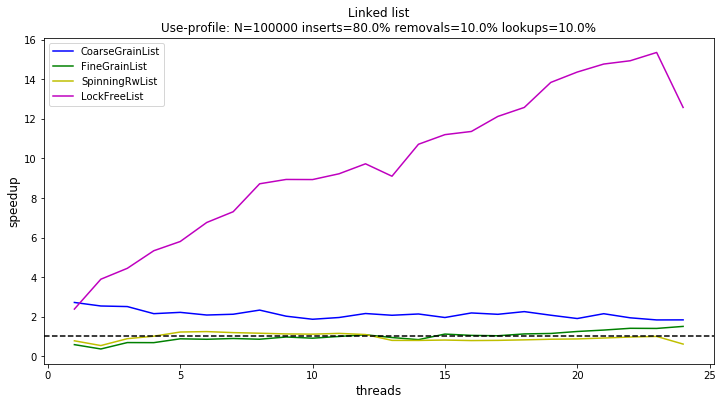
\includegraphics[width=1.0\linewidth]{figs/lateday/combined/lateday_combined_list_insert_80_lookup_10_removal_10}
\caption{
Speedup for concurrent lists with $N=100000$ and an insertion heavy workload:
80\% insertions, 10\% removals, and 10\% lookups.}
\label{fig:listInsertHeavy}
\end{figure}

\begin{figure}[h]
% ----- first row
\begin{subfigure}{.6\textwidth}
  \centering
  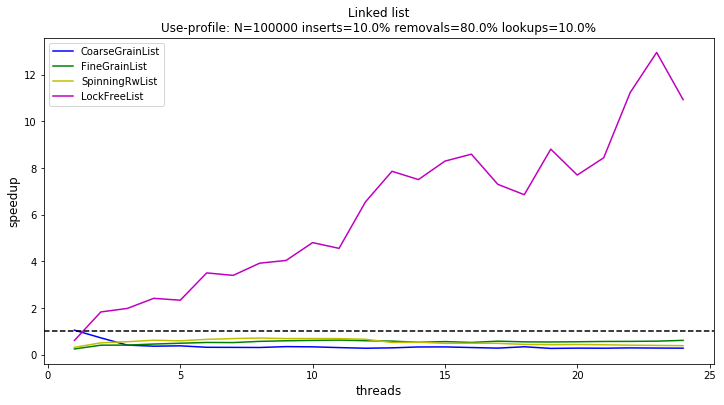
\includegraphics[width=.8\linewidth]{figs/lateday/combined/lateday_combined_list_insert_10_lookup_10_removal_80}
  \caption{Removal heavy workload.}
  \label{fig:listRemovalHeavy}
\end{subfigure}%
\begin{subfigure}{.6\textwidth}
  \centering
  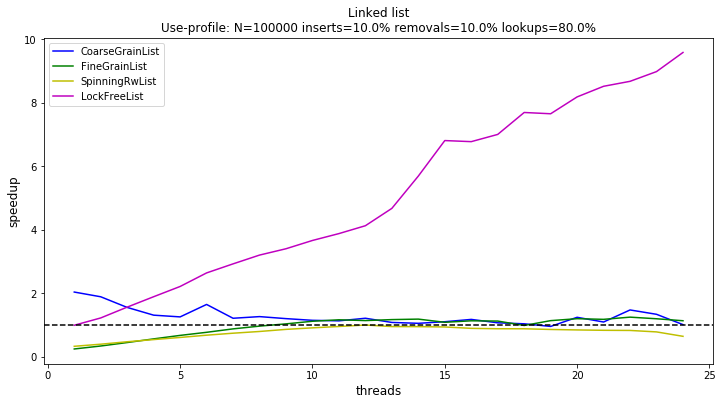
\includegraphics[width=.8\linewidth]{figs/lateday/combined/lateday_combined_list_insert_10_lookup_80_removal_10}
  \caption{Lookup heavy workload.}
  \label{fig:listLookupHeavy}
\end{subfigure}
\\ % ----- second row
\begin{subfigure}{.6\textwidth}
  \centering
  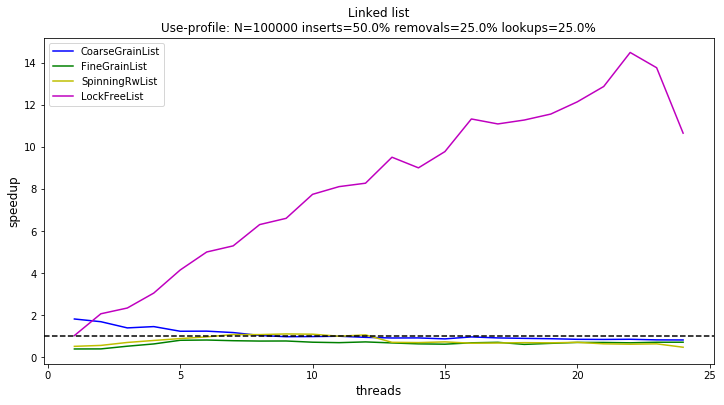
\includegraphics[width=.8\linewidth]{figs/lateday/combined/lateday_combined_list_insert_50_lookup_25_removal_25}
  \caption{Insert medium workload.}
  \label{fig:listInsertMedium}
\end{subfigure}%
\begin{subfigure}{.6\textwidth}
  \centering
  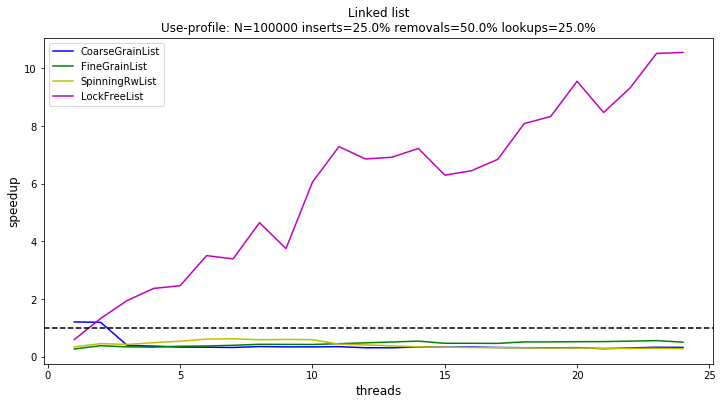
\includegraphics[width=.8\linewidth]{figs/lateday/combined/lateday_combined_list_insert_25_lookup_25_removal_50}
  \caption{Removal medium workload.}
  \label{fig:listRemovalMedium}
\end{subfigure}
\caption{
Concurrent list speedup with $N=100000$ and different use-profiles.
\ref{fig:listRemovalHeavy} has a use-profile of 10\% inserts, 10\% lookups, and
80\% removals. \ref{fig:listLookupHeavy} has a use-profile of 10\% inserts, 80\%
lookups, and 10\% removals. \ref{fig:listInsertMedium} has a use-profile of 50\%
inserts, 25\% lookups, and 25\% removals. \ref{fig:listRemovalMedium} has a
use-profile of 25\% inserts, 25\% lookups, and 50\% removals.
}
\label{fig:manyLists}
\end{figure}

\subsection{Hashmap results}

\section{Conclusion}

\section{Division of Work}
Equal work was performed by both partners.

\printbibliography

\end{document}
\grid
